\chapter{Environment}
\section{Foraging}
\label{sec:enviroment:foraging}

\begin{definition} \label{def:Welfare}
\textbf{Welfare} is defined as the state of wealth and can either be personal or collaborative (social).
\end{definition}

\begin{definition} \label{def:Maximising Social Welfare}
\textbf{Maximising Social Welfare} is a strategy which attempts to maximise the total amount of welfare (resources) the islands have.
\end{definition}

\begin{definition} \label{def:Stag Hunt}
\textbf{Stag hunt} or otherwise known as the assurance game or trust dilemma describes a conflict between safety and social cooperation
\end{definition}


\subsection{Foraging Background}

Foraging is a fundamental requirement required to obtain more resources during the simulation. It is based on the concept of inputting resources to get a return.

\subsubsection{Underlying Concept}

The primary objective of foraging in this game is to introduce a dilemma to the agents in order to investigate their behaviours and whether they work together despite different personal goals. Including two methods of foraging promotes decision making among the islands, allowing for strategic interactions to maximise personal benefits while still reaching the overarching goal of survival. 

The inspiration for our concept of foraging comes from the stag hunt game Definition~\ref{def:Stag Hunt}. Thus, it introduces elements from it. Specifically, this approach results in a game with \textbf{no dominant strategy} and in which \textbf{an agent's choice can impact another agent's}.

In the process of a stag hunt, each agent selects a method of hunting without the information of the other agents. The social welfare (total payoff) is significantly reduced if their choices differ. The selection of stag suggests that the agent is going for higher \textbf{payoffs} whilst the selection of hare indicates that the agent is \textbf{risk aversion} as both agents are required to stag hunt to get any personal welfare (see Definition~\ref{def:Welfare}).

\subsubsection{Modifications to the Original Underlying Concepts} 
A few changes have to be made to make this dilemma viable for our multi-agent system, in addition to adding realism. 

\begin{enumerate}
    \item The dependency was changed to be based on the input resources rather than the number of islands participating. This added a more realistic element to the dilemma as in reality a hunt’s return would be based on the amount of resources (different possible resources: people, food, water and materials) entered rather than the number of islands participating.
    \item Instead of a specified return, probabilistic return was implemented which adds a randomness element to the game to prevent pattern recognition. These probabilities can be tied to the population, disasters, forecasting and number of animals hunted.  
\end{enumerate}

Furthermore, the dynamics of our agents and allowing for a more complex decision-making interaction between islands and the environment have been explored. It is worth mentioning that some of these design ideas were implemented in the coursework. These changes have been made to make foraging more volatile and unpredictable, adding to the complexity of the system. This allows the teams to further evaluate the agents’ performance on observing and to use learned knowledge to take action.

\subsubsection{Tier System}

Deer hunting and fishing are divided into tiers, dependent on the total amount of input resources. Tiers represent the number of fish that can be caught in a given day, and the “zero” tier represents the cost associated with getting to the hunting location. Beyond the zero tier, the cost of catching another deer or fish will decrease as it is easier to catch the second animal than the first one, since the agents have already arrived at the hunting location. Therefore, if the agents do not even enough to reach the first tier, then they wouldn't get any returns. It should be noted there is a limit to how many animals the agents can catch in a given day.

The focus of fishing is to avoid risk at the expense of payoff. This means that all tier requirements are lower than those for the deers. However, the return is also lower thus if only one island goes fishing they are still expected to have a low return as long as they have enough resources to catch the first fish. Thus, the benefit of deer hunting is higher payoffs. However, these improved returns come at the cost of significantly higher tier thresholds. Therefore, it is possible for a single island to go deer hunting without enough resources to reach the hunting location leading to no return.

\begin{equation}
\text{Increments of catching $n$ animals}=
\left( \begin{array}{ll@{}}
n=0 \longrightarrow \Delta^0 = 1 \\
n=1 \longrightarrow \Delta^1 = 0.8^1 \\
n=2 \longrightarrow \Delta^2 = 0.8^2 = 0.64 \\
n=2 \longrightarrow \Delta^3 = 0.8^3 = 0.512 \\
n=4 \longrightarrow \Delta^4 = 0.8^4 = 0.4096\\
\end{array} \right) 
\label{eq:Cumulative Cost 1}
\end{equation}

\begin{equation}
\text{Utility Tier Cost}=\ \sum_{n=0}^{n} \Delta^{n} = \Delta^{0} + \Delta^{1} + \Delta^{2} + \Delta^{3} + \Delta^{4} + ....
\label{eq:Cumulative Cost 2}
\end{equation}

Equation~\eqref{eq:Cumulative Cost 1} and Equation~\eqref{eq:Cumulative Cost 2} show the formulation of the decay function for tier system. The tier system is shown in the Figure~\ref{fig:Foraging Tier System} where $n$ stands for the tiers, with decay costs ($\Delta$) of $0.8$ for the deer hunt and $0.6$ for fishing.

\begin{figure}[!htb]
    \centering
    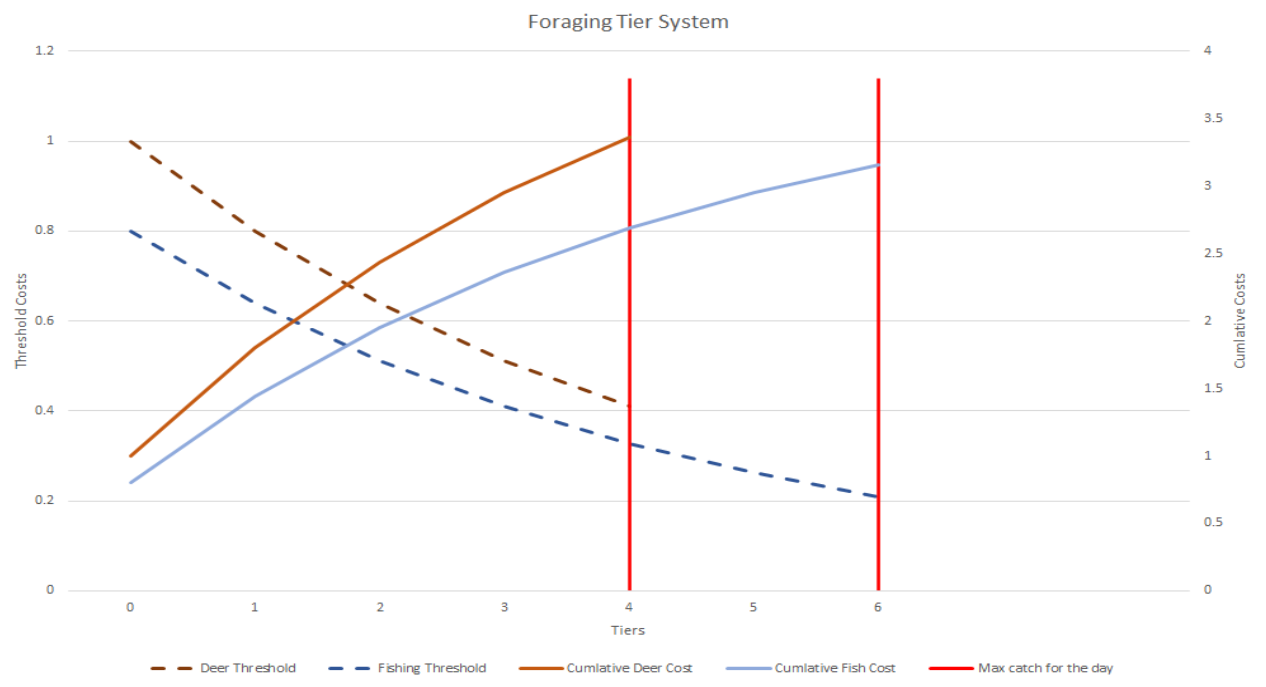
\includegraphics[width=0.9\textwidth]{04_environment/images/Foraging Tier System.PNG}
    \caption{Foraging Tier System}
    \label{fig:Foraging Tier System}
\end{figure}

The resources input are scaled using a variable and the tiers are then calculated with them, the higher the tiers the lower the cost to catch the next animal. However, the total cost increases up to a daily catch limit. This means that if teams collaborate, they can invest less as individuals to get a collectively greater return through deer hunting. If they invest too much, then they will over spend as they reach the daily catch limit. As a result, it is more beneficial for some teams to go fishing because it has a higher daily catch limit, although it comes with lower returns. In other words, there is a need for some self-sacrifice to reach the maximum welfare (see Definition~\ref{def:Welfare}). Moreover, fishing is a similar foraging method with the key difference being that it utilised a normal distribution and the start of the tiers.

\subsection{Example Distribution}
\subsubsection{Example of the Distribution for Foraging Return (Deer Hunting - Payoff Dominant)}

\begin{figure}[!htb]
    \centering
    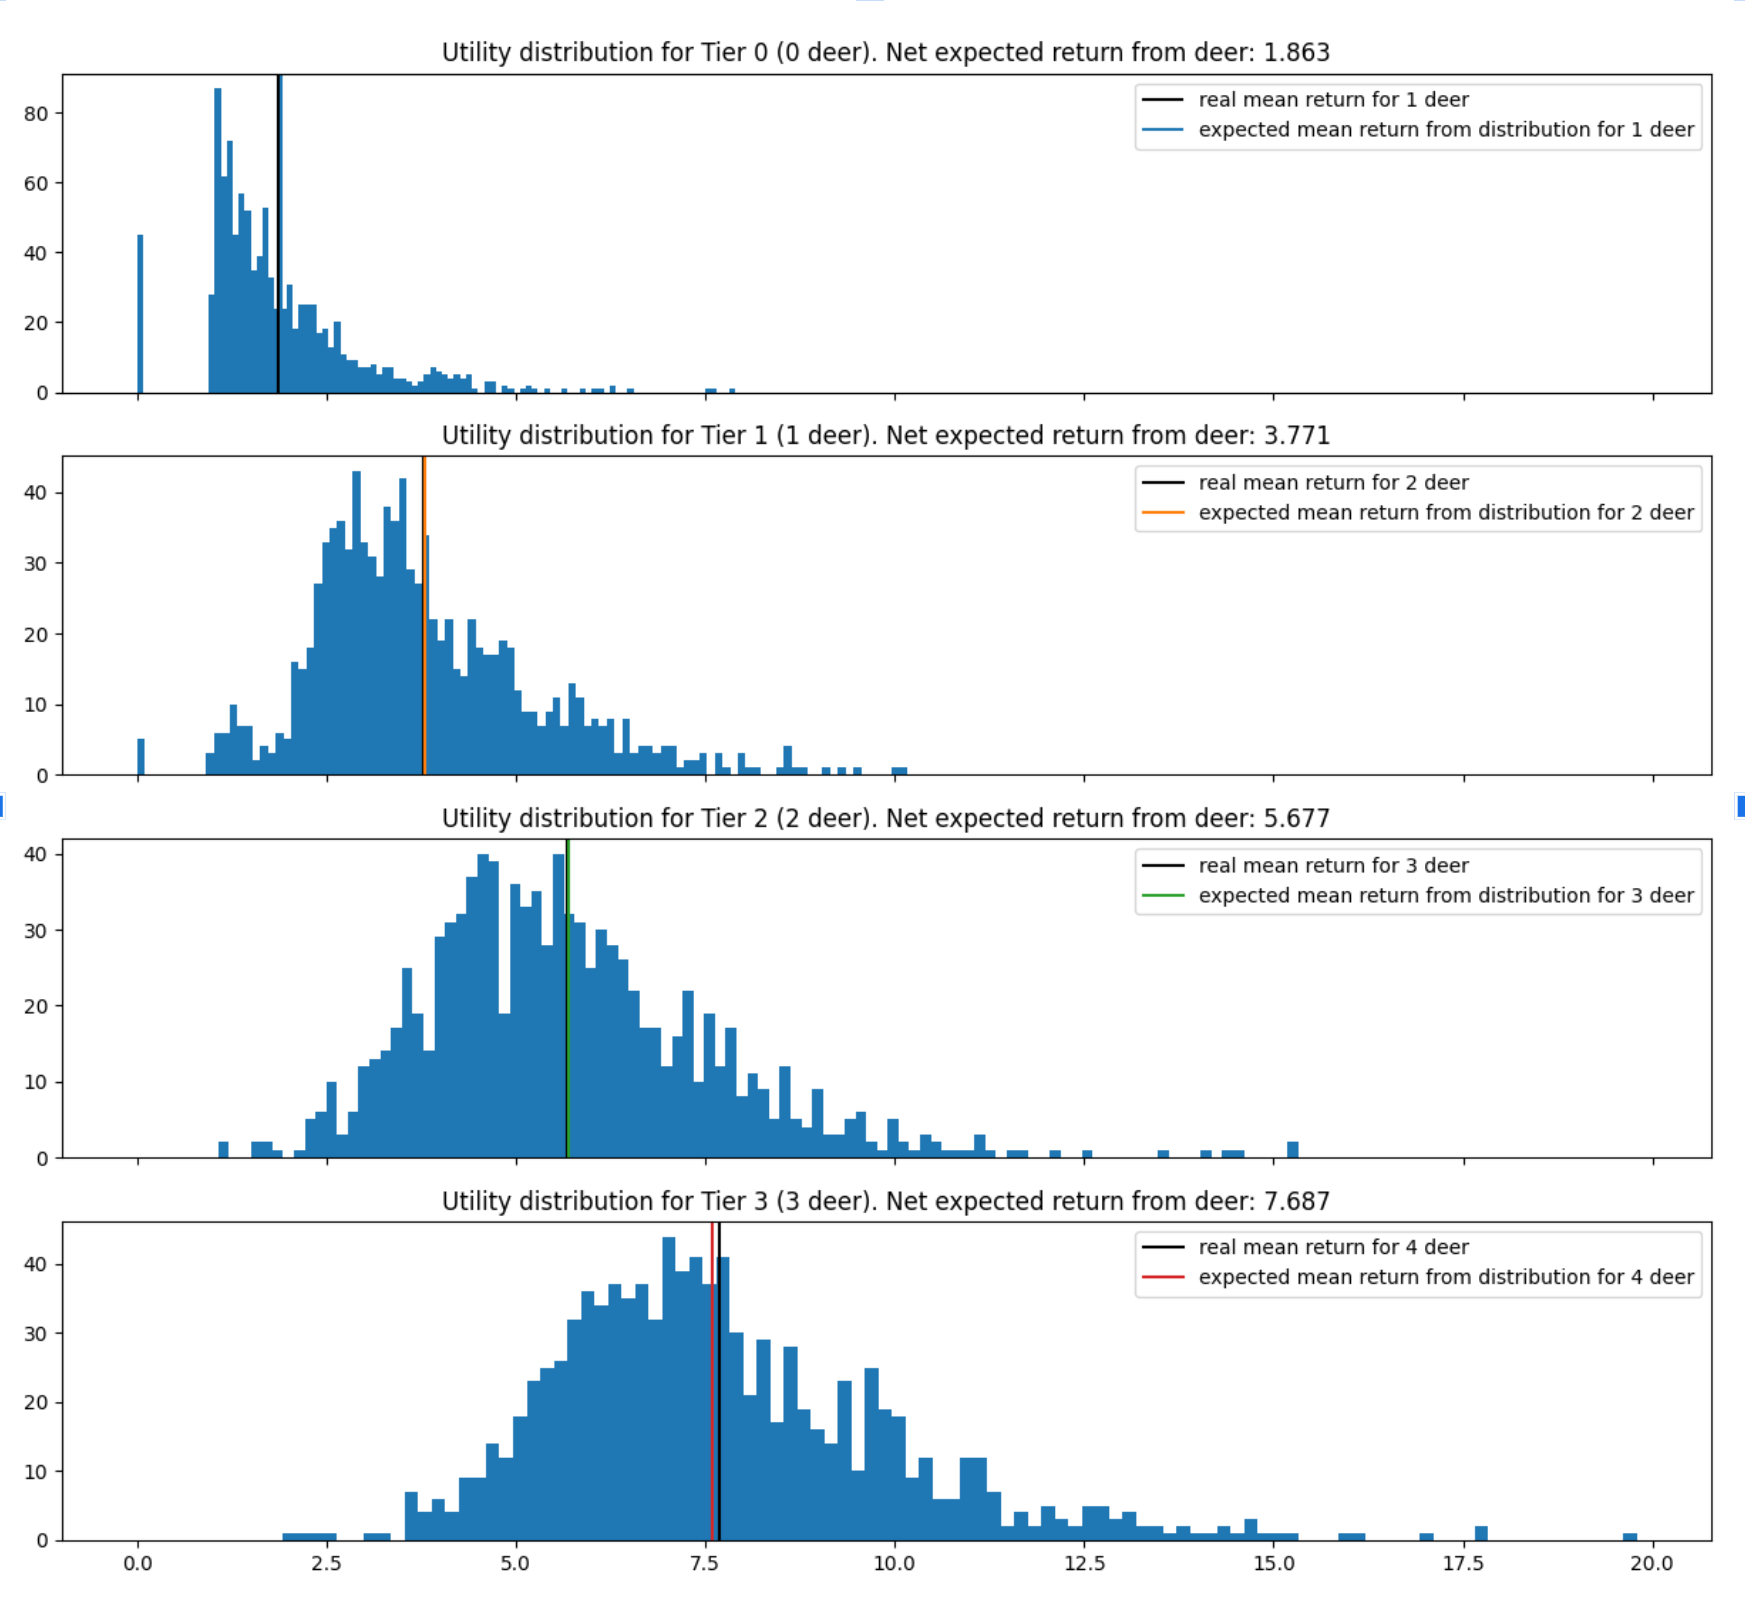
\includegraphics[width=1\textwidth]{04_environment/images/Distribution of Foraging returns Deer Hunting.PNG}
    \caption{Deer hunting payoff dominant Distribution for foraging return}
    \label{fig:Distribution of Foraging returns Deer Hunting}
\end{figure}

To increase the risk of deer hunting, a Bernoulli Random Variable ($D$) was used to prevent guaranteed resource returns after a hunt. The Exponential Decay ($W$) disincentives too many resources being allocated to hunting in the hope of a higher return. However, this all comes with the benefit of significantly higher ($2\times$) returns than fishing.

Figure~\ref{fig:Distribution of Foraging returns Deer Hunting} represents the return utility which will be multiplied by an output scale to give the return payoff. The Figure~\ref{fig:Distribution of Foraging returns Deer Hunting} shows the average \textbf{expected mean} return utility, in colour, after $1000$ iterations to be close to the \textbf{real mean}.

\newpage
\subsubsection{Fish hunting - Risk Aversion}

Fishing is similar to Deer hunting, except that it uses only a Normal Distribution ($F$), which focuses on avoiding risk by being very predictable and safe. Figure~\ref{fig:Distribution of Foraging returns Fishing} illustrates the return utility for fishing.

\begin{figure}[!htb]
    \centering
    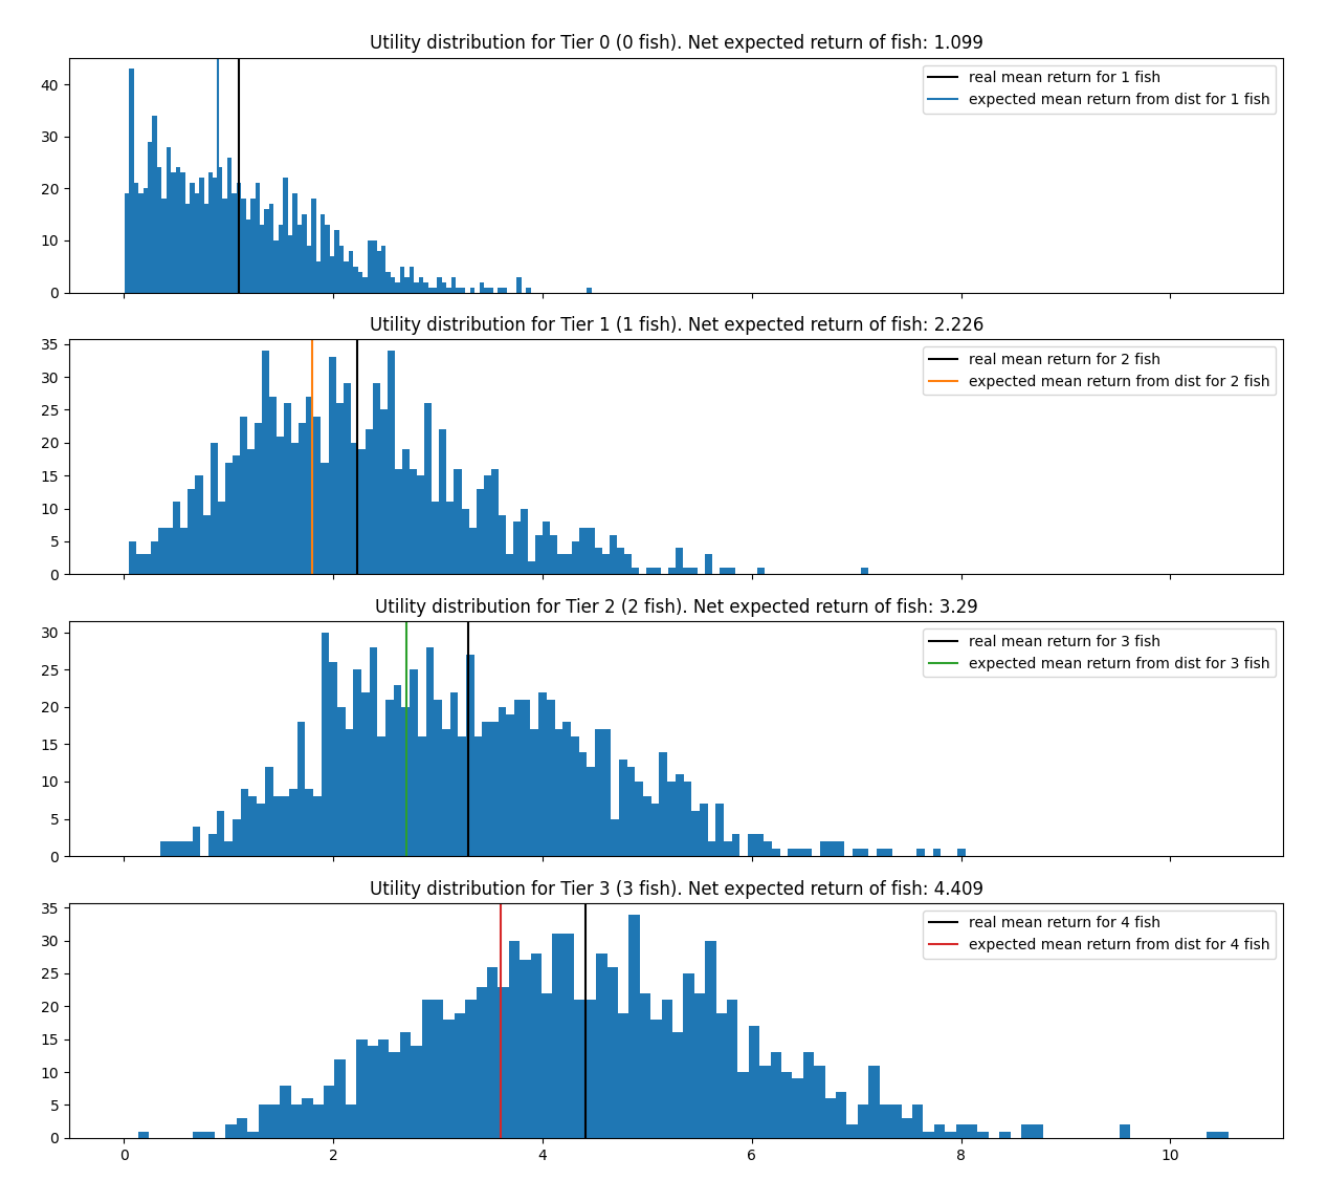
\includegraphics[width=1\textwidth]{04_environment/images/Distribution of Foraging returns Fishing.PNG}
    \caption{Fishing Risk aversion Distribution for foraging return}
    \label{fig:Distribution of Foraging returns Fishing}
\end{figure}

As seen in Figure~\ref{fig:Distribution of Foraging returns Deer Hunting} and Figure~\ref{fig:Distribution of Foraging returns Fishing}, the return for the deer is almost double that of the fish return whilst the fish return is much easier to obtain due to the lower cost of catching fish.

\newpage
\subsection{Solution Concepts}
\subsubsection{Dominant Strategy}

In this implementation, there is no dominant strategy. Therefore, if an agent decides to go deer hunting, whereas all the other islands are fishing, that agent would not get the best return possible. It is not the best strategy. Whilst if an agent goes fishing and there are a sufficient amount of agents deer hunting, then that agent would be passing on the opportunity of to gain a larger return in deer hunting. Hence, it is not the best strategy either.

\subsubsection{Nash Equilibrium}

In the regular stag hunt game, there are two pure Nash Equilibria, where both agents go for either payoff or risk aversion. In our implementation, there are multiple Nash Equilibria. These are the points where the islands cannot benefit themselves by moving to deers hunting to generate more return. As there is a limit to how many deers that can be hunted thus by moving to deer hunting they are getting a worse return than if they just stayed at fishing. Whilst the islands at the deer hunt are already making a greater return and have no reason to switch to fishing.

\subsubsection{Pareto Optimal Strategy}

At some point, all agents will be in a position where changing foraging methods will not yield any better income for themselves and in fact also hinder others. This is due to the max daily deer hunt limit which creates a maxim return on the deer hunt. Therefore there will be points where the islands will change as the amount of resources being entered into both methods of foraging is the most efficient, this being where deer returns are maximised. There may also be a point where the agent can benefit by switching away from deer hunting. However, this will cause the other islands in the deer hunt to have a worse pay off due to a possible drop in tier resulting in worse returns.

\begin{figure}[!htb]
    \centering
    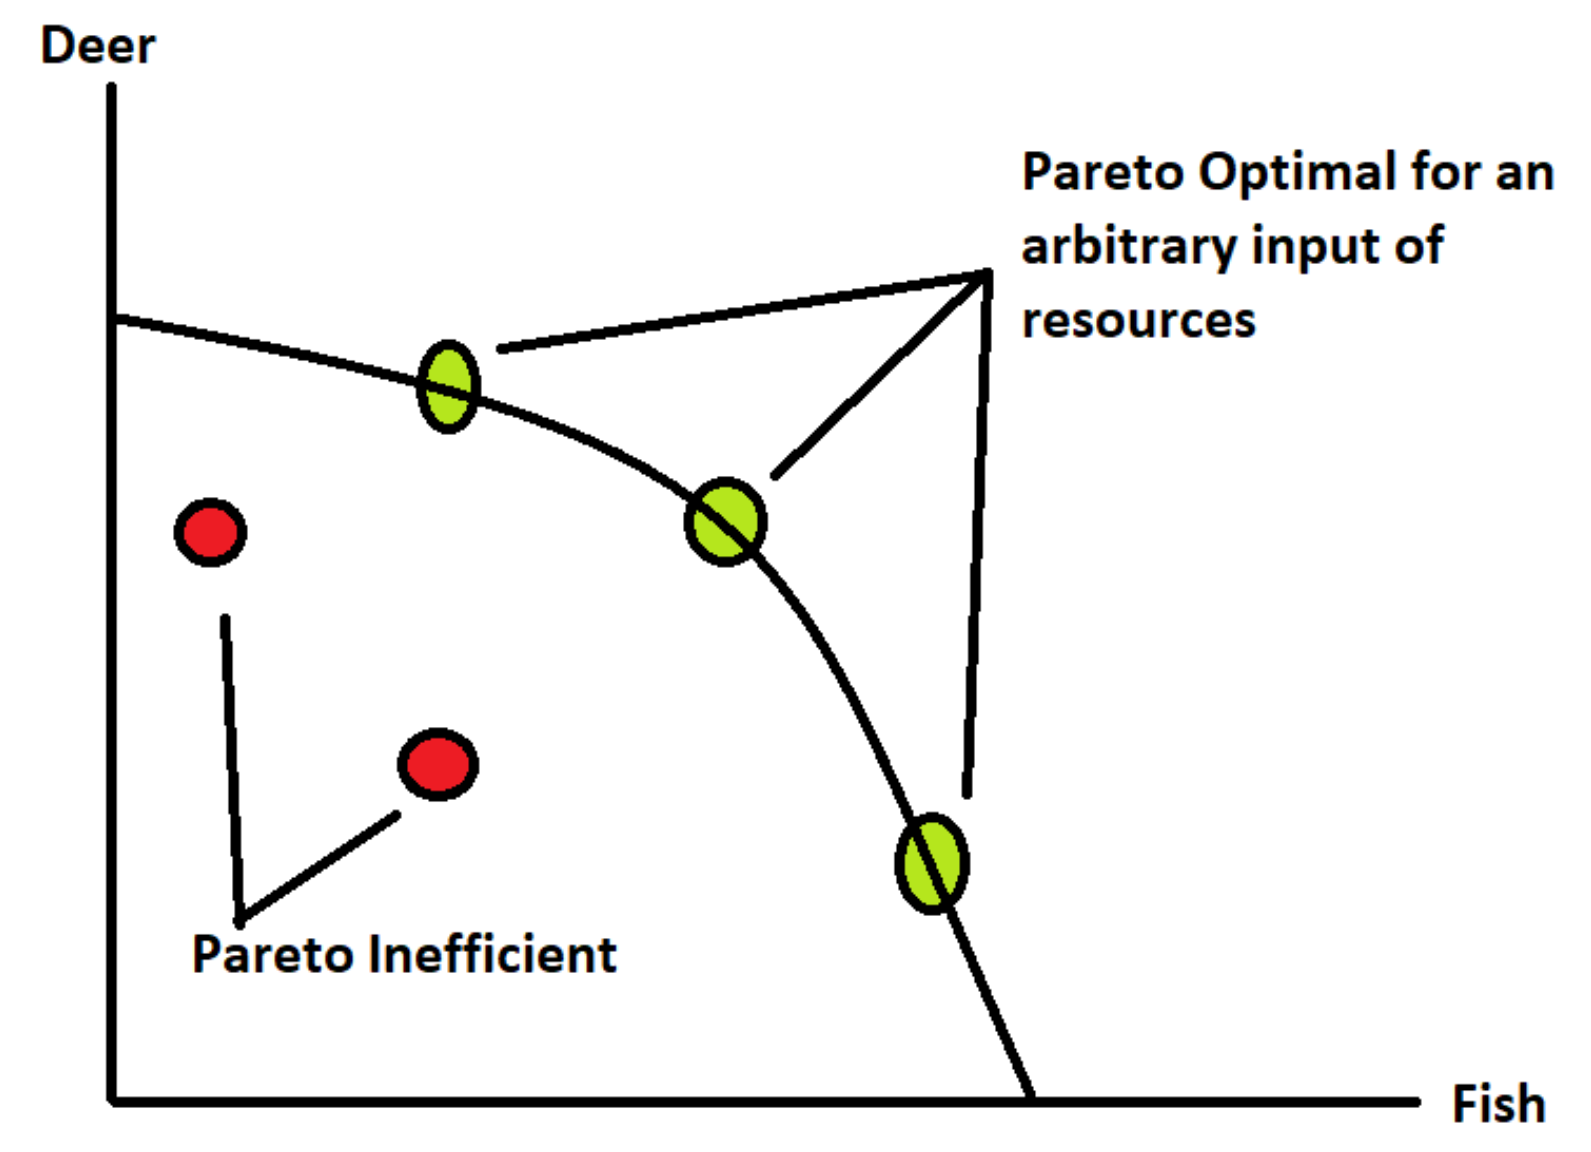
\includegraphics[width=0.7\textwidth]{04_environment/images/Pareto Optimal Strategy.PNG}
    \caption{Pareto Optimal Strategy}
    \label{fig:Pareto Optimal Strategy}
\end{figure}

\subsubsection{Social Welfare Maximisation}

It is possible for these islands to find the social welfare maximum (see Definition~\ref{def:Maximising Social Welfare}) in this foraging function with enough time. The islands could identify the exact amount of resources needed, for both fishing and deer hunting, to achieve the best return according to the maximum number of animals. Thus, by cooperating who goes where and spends how much, they are able to maximize their returns without spending more resources than necessary.

\subsubsection{Population Density}

Introducing a model that controls the population density of deer allows us to increase the complexity of the foraging function. In short, the deer hunting capacity decreases with decreasing population and increases with an increasing population. This then influences the maximum deer per hunt parameter ($n$), which in turn results in a more complex return calculation function (\texttt{\textbf{DtotalReturn}}), which would make it harder for agents to figure out forage tier boundaries to optimise their strategies.

The population change can be dynamic depending on various environmental factors. For example, a disaster could supposedly cause the population density of deer to halve, making it harder to forage and therefore, causing lower returns. In this current implementation, a single species population model and more specifically logistic modelling for the deer and fish population was implemented. 
The model is described in Equation~\eqref{eq:Population Density}.

\begin{equation}
\frac{\mathrm{d} P}{\mathrm{~d} t}=k(N-P)
\label{eq:Population Density}
\end{equation}

\begin{itemize}
    \item $P$ is the total population. 
    \item $N$ is the maximum deer population (carrying capacity\footnote{The maximum population size of a biological species that can be sustained in a specific environment.}).
    \item $k$ is the growth coefficient.
    \item $t$ is time.
\end{itemize}

In Figure~\ref{fig:Deer population over time}, the simulation of the implemented logistic model can be observed, with a growth coefficient of $0.2$ and $N$ of 8. It can be seen that there is an unpredictable pattern to population changes, which would be interesting to see affecting the tier system and in extend, the deer and fish foraging strategies of the agents.

\begin{figure}[!htb]
    \centering
    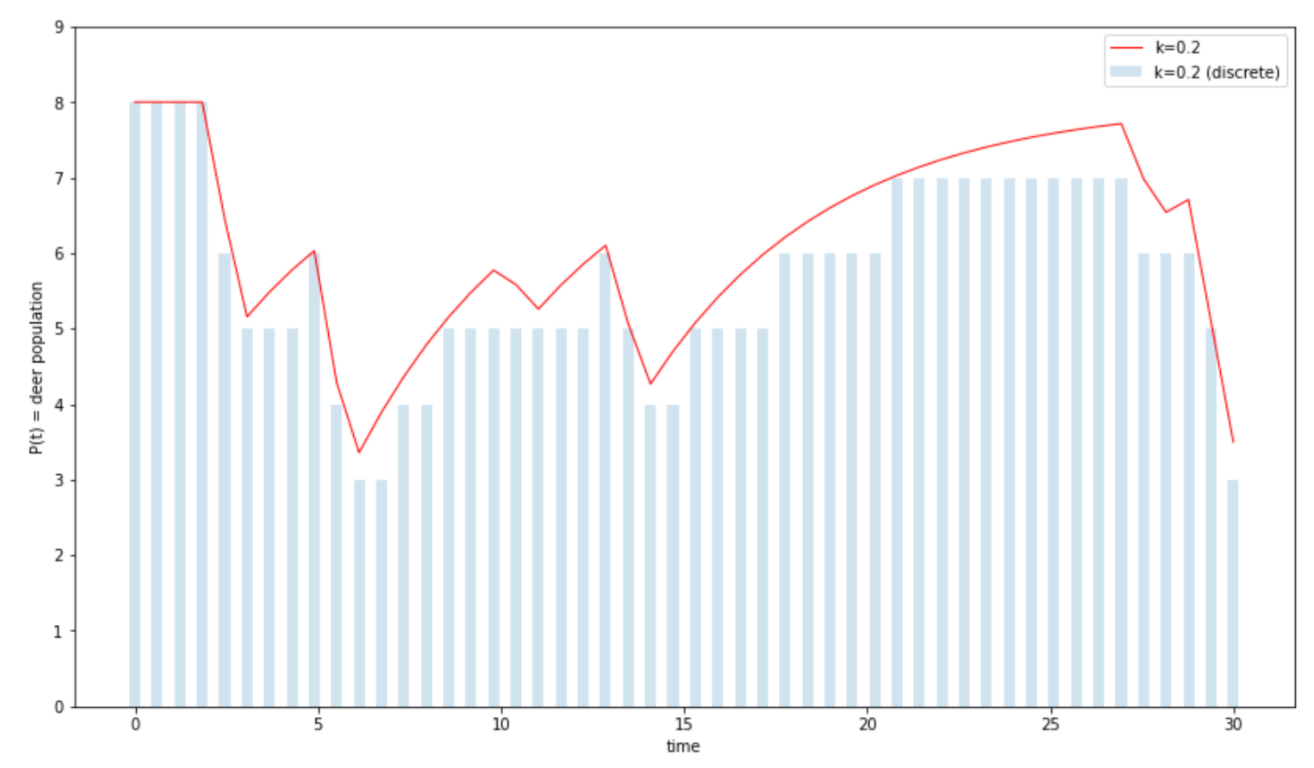
\includegraphics[width=1\textwidth]{04_environment/images/Deer population over time.PNG}
    \caption{Deer population over time (turns) under Logistic modelling with a growth coefficient of 0.2.}
    \label{fig:Deer population over time}
\end{figure}

Furthermore, In our implementation, $k$ and $N$ are constants. 

Modelling the population (or linking it to other environmental elements) allows us to make sure that the system’s dynamics are varying, making it harder for islands to settle onto a single foraging method because it always results in better returns. Pareto optimality is therefore harder to achieve and thus maximising social welfare (see Definition~\ref{def:Maximising Social Welfare}) is trickier, requiring agents to make more informed decisions, recognizing possible patterns. Of course, that would be an easier task for the islands, if they had knowledge on what is affecting the population (i.e. disasters), whereas a logistic model function might be more abstract in the eyes of our agents, requiring more processing. 

\subsubsection{Method of Resource Allocation}

Moreover, there is a parameter to allow either an equal split of returns after foraging regardless of the input, or a proportional split dependent on the amount of resources inputted by each island. Both of these implementations work in accordance to the previous specification. Such change allows us to observe the concept of free-riding further, looking at how greedy islands behave in the case of uniform resource returns.

The distribution method is based on two scalars. The first scalar is to scale input resources into tiers, allow the user to choose how much they wish. After which, the number of fish or deer caught is chosen by the tiers which goes into their respective distributions. The output of these distributions are then multiplied by the second output scalar. This allows the user to adjust the return amount each island can obtain, the output scalar should be above the cost of living in order to ensure the islands have enough resources to survive.  

\subsection{Future Work}

Further work could be done to make sure that there is enough complexity to explore the dynamics of our agents. Due to the project’s time constraints, some interesting ideas were not implemented but were thoroughly examined during the design process.

An important add-on to our previous implementation could be the enforcement of laws by the IIGO for the number of islands that can go foraging. That would introduce the need of internal agent relationships, adding another level of decision-making complexity to the agents. The specific alteration could result in some interesting findings. For example, there could be an auction scenario where islands would bid with their input resources, where only the highest bidders would be able to forage, as limited by the IIGO. Therefore, the islands with the lowest resources would be out-bidded, possibly causing a long-term resource depletion that would need to be mitigated by the more resourceful islands later in the game. It would be interesting to see how such change would affect the free-rider problem and how islands would adjust their strategies to out-bid other islands.

Another change that could be made is to let islands choose who they want to forage with. The islands would communicate with each other in form of direct messaging or voting to reach a decision. Essentially, our speculation is that agents would avoid the free-riding problem in both cases by enabling agents to make collective decisions based on communicated resource contributions. That’s because free-riders would be out-voted or not invited for foraging. That, in combination with the aforementioned tier system, would possibly result in all the islands contributing as much as possible to the input foraging “pool”. However, it would be interesting to see if islands can then reach Pareto optimality, where every single agent gets the best possible return for their input.

In addition to the above suggestions, agents would be restricted to just a single foraging area where they would only be allowed to forage with one neighbouring island using a ranking algorithm. This could alter the game's dynamics as an agent would only have limited partners (i.e. other islands) to forage with i.e. other islands in the same limited area. The aforementioned islands could be explicitly decided or randomly allocated. This could also be enforced and implemented as future work. Moreover, this particular scenario could be extended by programming prey densities to be geo-focused, where prey populations could vary between regions on the “map”. Islands would then need to make a strategic plan on how their ranking of neighbouring islands would change in accordance to their returns and returns broadcasted from other island pairs.

As discussed earlier, the population density of deer is a parameter that allows us to increase the complexity of the foraging function, tying it up to a realistic population model. It would be interesting to see what would happen if the growth coefficient increases, causing a population growth and observing the islands’ dynamics. Will they keep on “investing” higher resources each turn, taking advantage of the deer and fish abundance, or will they stick to their original, safe and static strategy?

In addition, going into resource allocation, the utility is in fact multiplied by an output multiplier. Therefore, the user determines the output multiplier value, as well as the resource allocation. Thus, agents can receive either a proportional split or an equal allocation of resources based on the users' decisions. Moreover, a few questions that be could be asked about the islands relationship and behaviour are: Will the islands seek to minimise inputs and benefit from the more generous islands, even at the cost of being allocated a lower tier? Will they input just enough to maximise the tier they are foraging in? Or, will they observe other island’s previous contributions and make a decision based on that?

Finally, more foraging options could be added in future implementations. For example, a third foraging technique; whale hunting could be created. This option would have an even higher return than deer hunting, deeming it an appealing forage method. The barriers of entry could be similar to that of the deer hunting method in this scenario but at the same time, there would be a more spaced out/expensive tier system. This combination would potentially incentivise cooperation between islands, if their strategy was to maximise returns. Also, as additional foraging methods have been introduced, the type of return was fixed for each foraging method and observe how agents decide to behave. For example, the deer and fish hunting methods result in returns proportional to inputs, whereas the whale hunting method would result in an equal split of returns between all participating islands. Would this mean that islands choose a fairer division of returns and not go on whale foraging at all? Or would they be intrigued by the higher costs and choose whale hunting over the other foraging methods? In the latter question, agents would need to take into account that an island may enter an insignificant amount of resources and reap a large return. It is therefore up to the islands to decide if the higher payoff is worth the risk of other islands free-riding.

All the aforementioned behaviours are, of course, influenced by the island tactics. Therefore, an island programmed to be greedy could not cease to be greedy, no matter how the surrounding islands’ behaviours change, unless the greedy island can adapt. Therefore, agent strategies must attempt to draw conclusions on specific foraging methods and modify their strategies where appropriate.

\newpage
\section{Disaster}
\subsection{Disaster Background}

A game was designed where agents directly confront a disaster and its risks once every round. This subset of the game creates a dilemma, where each island (agent) has to survive. They will have the opportunity to work together by investing collectively to the common pool, the disaster will be mitigated if the islands invest enough resources to reach a desired threshold. Otherwise, the islands would face negative impact, which would diminish their available resources. It is worth mentioning that the disaster will first extract resources from the common pool, and then if not enough resources have been invested, resources will be depleted from each island proportionally to their island’s damage.

Furthermore, the disaster was designed to comprise of an epicentre (eye of the storm), which is limited within the archipelago bounds, it is represented using Cartesian coordinates $(EpiX, EpiY)$. Therefore, all islands or a subset of islands may be affected due to their proximity to the disaster epicentre. The island’s proximity to the disaster epicentre is directly proportional to the island’s damage. In other words, the island's available resources will be diminished based on the disaster magnitude and its location with respect to each island’s fixed location.

The following example can briefly explain the dilemma:

The closest an island from the eye of the storm, the larger the severity on that island. Therefore, the more resources are depleted. Let’s say the disaster epicentre hits around Island 1 as shown in Figure~\ref{fig:Disaster eye of the storm severity} and that the desired common pool threshold has not been met. Island 1 would be experiencing severe damages , and Island 2 and 6 some damages and the other islands low to no damage. Therefore, Island 1, 2 and 6 have the risk of not surviving if they are lacking resources, whereas Island 3, 4, and 5 would not be affected as much by the disaster.

\begin{figure}[!htb]
    \centering
    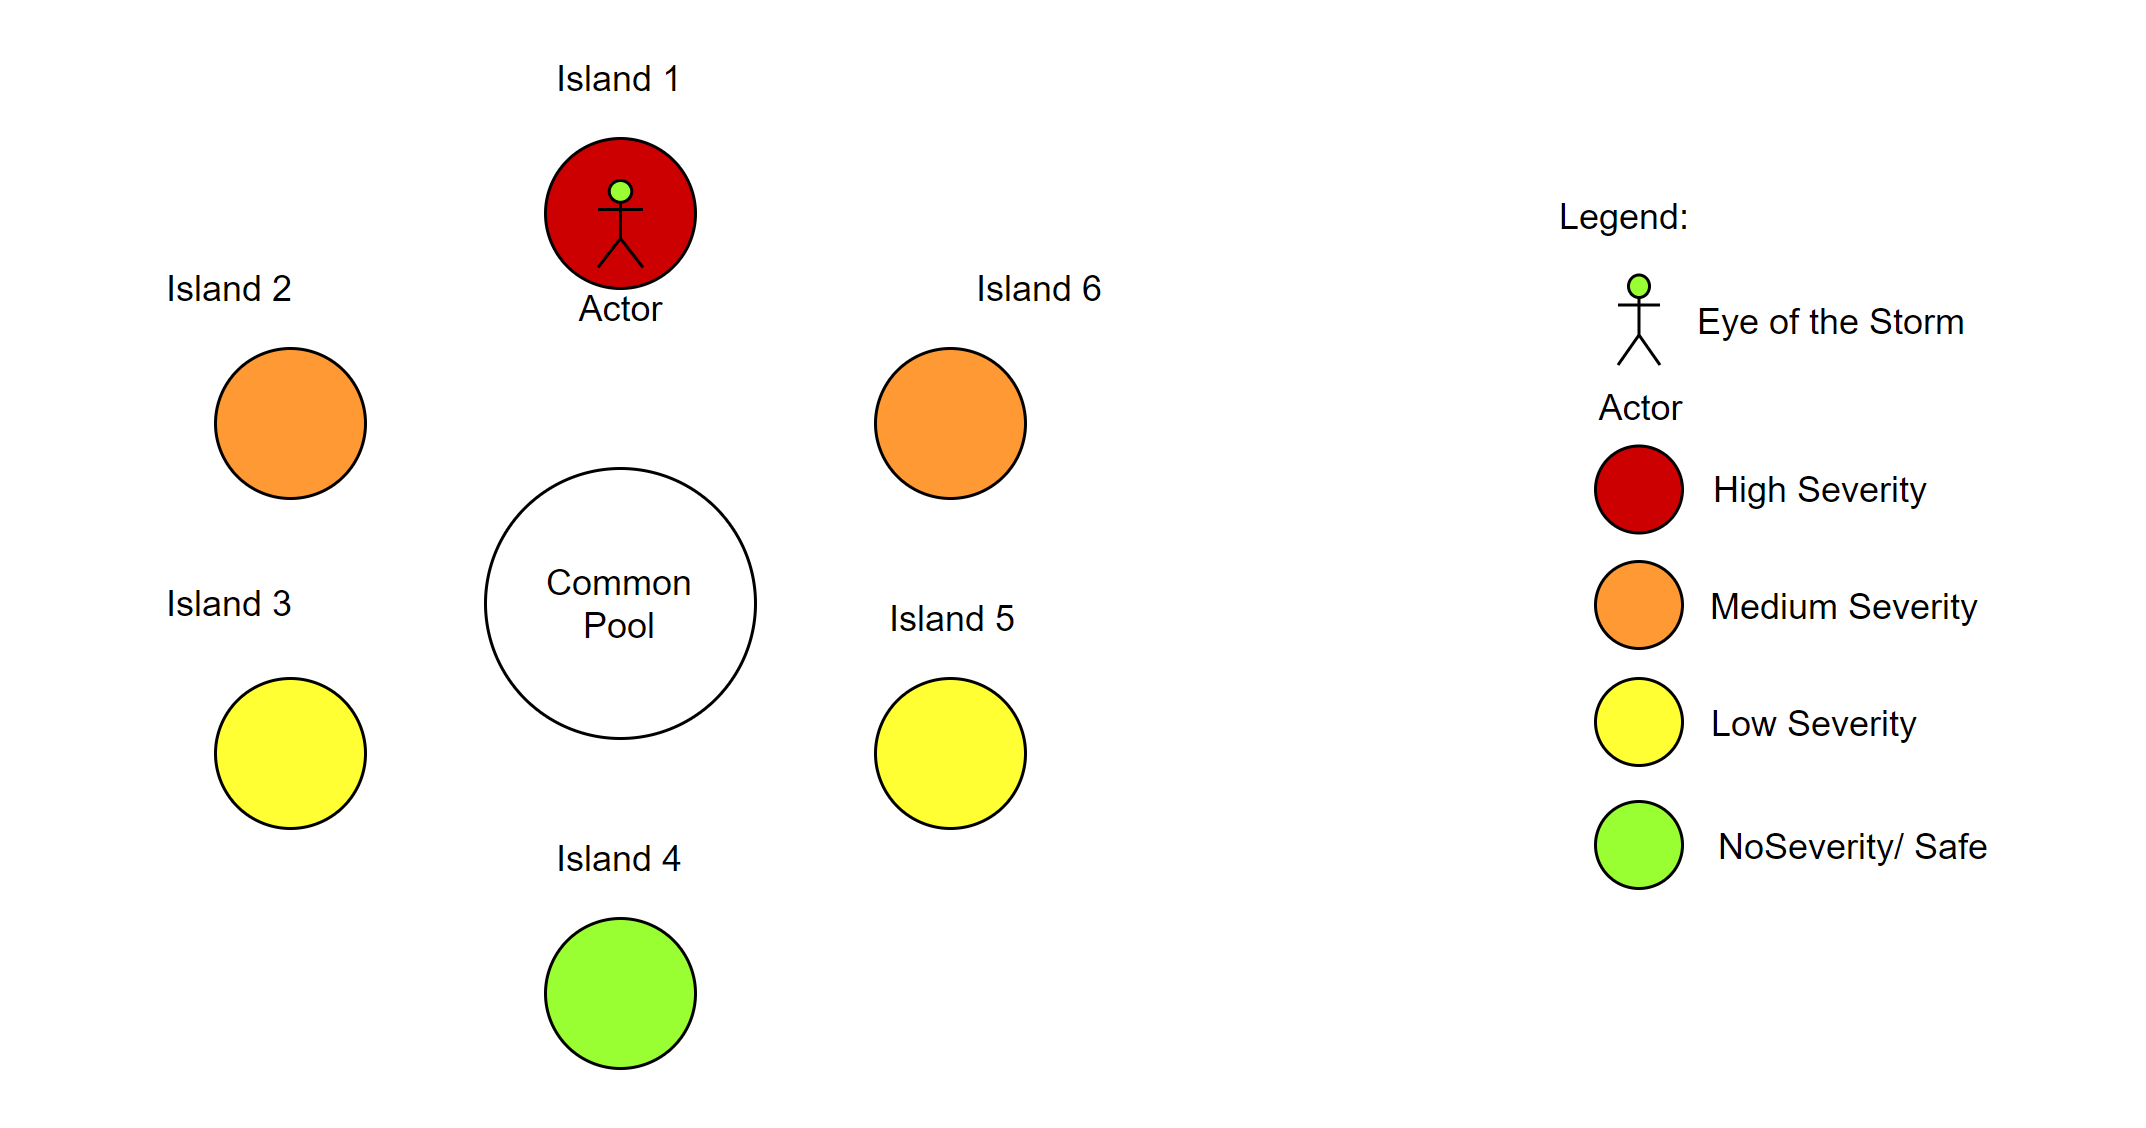
\includegraphics[width=1\textwidth]{04_environment/images/Disaster eye of the storm severity.PNG}
    \caption{Disaster Epicenter effects}
    \label{fig:Disaster eye of the storm severity}
\end{figure}

\newpage
\subsection{Future work}

There are multiple future work ideas that would be developed in the design aspect such as; a deterministic disaster which would be  designed as a straight line that accumulates during the days, once the threshold was met then the disaster would occur. Another deterministic disaster idea would be to link the disaster’s magnitude to time. Thus, agents would have to learn from past disaster occurrences, creating a memory. Agents would start learning from past disasters and would be able to forecast the next one. Therefore, the agents would be able to forecast that if a disaster did not surface for a long period of time, then the magnitude of the next disaster will be much larger than the previous one.

Another idea is that agents can invest into forecasting. Therefore, agents will have access to a history of past disasters, which would be utilised to learn and gain knowledge in order to predict the upcoming disasters. Thus, the more resources invested by the agents in forecasting, the more disaster history data will be provided. This would enable the agents, to apply machine learning techniques to such data, allowing them to acquire more accurate and precise predictions of future events and develop better risk assessments. Therefore, agents will acquire knowledge, when investing in any of their resources.


\section{Common Pool}
\subsection{Common Pool Background}

A game was designed where one group of six islands (agents) have access to a common-pool resource. In micro-level, each island intends to maximise its utility while in macro-level, all the islands want to maintain sustainability and be protected by the upcoming disaster. The above description specifies a collective action problem where n-agents (six in our case) are seeking access to a common pool resource that is sufficient to satisfy some agents but not to satisfy all of them.

A Linear Public Goods (LPG) Game was implemented, where all the agents individually own some resources and try to maintain and increase them, by foraging, but also contribute a part of them to the common pool. This common pool is used for the payment of expenses of the institutional roles and for the protection towards the disaster.

In more detail, the common pool is represented by a structure with following characteristics:

\begin{itemize}
    \item Common Pool Threshold.
    \item Amount of Resources.
\end{itemize}

According to the specifications of a Linear Public Goods Game, the agents should be able to perform the following actions:  

\begin{itemize}
    \item Request Resource from the Common Pool.
    \item Contribute Resource to the Common Pool. 
\end{itemize}

And the Common Pool is responsible for two more actions: 

\begin{itemize}
    \item Mitigate disaster.
    \item Deplete islands after a disaster.
\end{itemize}

The common pool threshold is a fixed value and known to islands and its resources will be given to each island based on the severity of the damages. If the amount of resources in the common pool exceeds the total effect of disaster, then the leftover amount of resources in the common pool will be used for the next round. Since the goal of each island is to maximise its utility, the following dilemma shows up: islands can free ride by not contributing to the common pool and yet receiving the benefits after a disaster or if they are aware that they would not be depleted by the disaster - since they are far away from the eye of the storm - they might also not contribute to the common pool and thus the rest of the islands would be severely destroyed.

The following example can briefly explain this dilemma:

If the epicentre of disaster is known to the islands and happens to coincide with the location of Island 1, then Island 4 might not contribute at all to the Common Pool since it will not be affected by the disaster. Moreover, Islands 3 and 5 that will not be severely hit might contribute a small amount to the Common Pool or even zero amount (free riding case). Since the rest of the islands might contribute to the Common Pool, then Islands 3 and 5 will be profited by the contribution of others.

importance of prevention and incentivise islands to contribute to the Common Pool is highlighted, thus if the amount of resources in the common pool exceeds the threshold when the disaster happens, then the “power” of disaster towards the islands and common pool will be decreased. It makes sense in real life, as more preparation will result in less damage. The actual damage of disaster is decreased by half.

\subsection{Example Distribution}
This can be described by the examples in Table~\ref{tab:Demonstration of how the common pool work in different scenarios}, which shows 4 possible scenario:

\begin{itemize}
    \item Contribution to common pool \textit{does not meet} threshold and common pool \textit{cannot} fully mitigate disaster’s damage.
    \item Contribution to common pool \textit{does not meet} threshold but common pool \textit{can} fully mitigate disaster’s damage.
    \item Contribution to common pool \textit{meets} threshold but common pool \textit{cannot} fully mitigate disaster’s damage.
    \item Contribution to common pool meets\textit{} threshold and common pool \textit{can} fully mitigate disaster’s damage.
\end{itemize}

\begin{table}[!htb]
\begin{center}
\begin{tabular}{|l|c|c|c|c|}
\hline
                               & \textbf{Scenario 1} & \textbf{Scenario 2} & \textbf{Scenario 3} & \textbf{Scenario 4} \\ \hline
\textbf{Disaster Total Damage} & 1000                & 200                 & 1200                & 1200                \\ \hline
\textbf{CP's Threshold}        & 500                 & 500                 & 500                 & 500                 \\ \hline
\textbf{CP's Current Value}    & 300                 & 300                 & 500                 & 700                 \\ \hline
\textbf{CP's Multiplier}       & 1                   & 1                   & 0.5                 & 0.5                 \\ \hline
\textbf{Mitigated Damage}      & 300                 & 200                 & 500                 & 1200                \\ \hline
\textbf{Remaining Damage}      & 700                 & 0                   & 100                 & 0                   \\ \hline
\textbf{CP's Remaining Value}  & 0                   & 100                 & 0                   & 100                 \\ \hline
\end{tabular}
\end{center}
\caption{Demonstration of how the common pool work in different scenarios}
\label{tab:Demonstration of how the common pool work in different scenarios}
\end{table}

\begin{itemize}
    \item In scenario 1, the disaster total damage is high. However, there is no preparation from the islands through contribution to the common pool. As a result, the common pool could not mitigate all of the damage and $70\%$ of the damage will be directly on the islands.
    \item In scenario 2, even though there is no preparation, the common pool is still able to mitigate all of the damage thanks to the low damage of disaster. The leftover resource in the common pool will stay there.
    \item In scenario 3, the disaster damage is high. Fortunately, the islands have prepared themselves moderately through contribution to the common pool. Thus, the islands only have to take very little leftover damage.
    \item In scenario 4, the disaster damage is high, and the islands have prepared themselves very well. As a result, the damage is fully mitigated by the common pool, and there is still leftover resource in the pool. 
\end{itemize}


\subsection{Future Work}

To observe behaviors of agents in different settings, the future work on the common pool could be centered around varying the values of different parameters such as threshold and threshold multiplier. The forecasting function of the disaster part can be used as a tool to variate the common pool’s threshold and multiplier accordingly. In events that damage could be high, the preparation should be done more carefully, thus the common pool’s threshold can be raised to let islands know about potential damage from disaster. The same thing can be done for threshold multiplier, where the multiplier will be greater for bigger disaster. Since threshold and multiplier both encourage the preparation for disaster, one of them can be fixed at certain seasons to observe different behavior of agents when it comes to varying different parameters. It is worth mentioning that the functionality of making the threshold unknown to the islands would be implemented in our future work.